\section{A point pole on the Hopf manifold}
\label{sec:hopf-point-equilibrium}

The one-point case on the Hopf manifold admits an explicit calculation of both the kernel measure and its Fubini--Study potential. It supplies a lower asymptotic for a selecting weight which does not descend. The limit also shows exactly which singularity information the section spaces have lost.

Use $X_n\to\mathbb P^q$, $q=n-1\geq1$, with $L=L_1$, the Fubini--Study metric and probability volume $\nu_X=\omega^n/(2n)$ from the preceding sections. Let $p\in X_n$ lie over $b=[1:0:\cdots:0]$. Suppose $\varphi$ has a single logarithmic pole of rational coefficient $0<a<1$ at $p$ and is locally bounded elsewhere, as in \eqref{eq:isolated-selecting-poles}. The continuous weight is zero. Set
\[
 \begin{gathered}
 t([Z_0:\cdots:Z_q])=
       \frac{|Z_1|^2+\cdots+|Z_q|^2}{|Z_0|^2+\cdots+|Z_q|^2},\\
 r_m=\max\{\lfloor ma\rfloor-q,0\},
 \qquad D_m=\binom{m+q}{q}.
 \end{gathered}
\]
Thus $t=0$ exactly at $b$. Define the function $e_a$ on $[0,1]$ by
\begin{equation}\label{eq:point-equilibrium-function}
 e_a(t)=
 \begin{cases}
 a\log(t/a)+(1-a)\log((1-t)/(1-a)),&0<t<a,\\
 0,&a\leq t\leq1,\\
 -\infty,&t=0,
 \end{cases}
\end{equation}
and put $E_a=e_a\circ t$ on $\mathbb P^q$. When $q=1$, this is the same function as $\Gamma_a$ in \eqref{eq:pone-explicit-model}; here it arises from a point pole on the total space of the fibration.

\Needspace{16\baselineskip}
\begin{proposition}\label{prop:hopf-point-binomial-kernel}
The selected kernel and dimension are
\[
 B_{X_n,m}=D_m\left(
          \sum_{j=r_m}^{m}\binom mj t^j(1-t)^{m-j}\right)\circ\pi,
 \qquad
 N_m=D_m-\binom{r_m+q-1}{q}.
\]
The last binomial coefficient is zero when $r_m=0$. In particular all these spaces are nonempty, and
\[
 \lim_{m\to\infty}\frac{q!N_m}{m^q}=1-a^q>0.
\]
\end{proposition}
\begin{proof}
By \cref{prop:isolated-pole-section-descent}, the space on the base consists of homogeneous polynomials of degree $m$ vanishing to order at least $r_m$ at $b$. In the affine chart $Z_0=1$, this selects exactly the monomials $Z^\ell$ with $\ell_1+\cdots+\ell_q\geq r_m$.

Coordinate circle invariance makes distinct monomials orthogonal. Their squared norms for $\sigma^q$ are
\[
 \int_{\mathbb P^q}\frac{|Z^\ell|^2}{|Z|^{2m}}\,\sigma^q
       =\frac{q!\,\ell_0!\cdots\ell_q!}{(m+q)!},
 \qquad |\ell|=m.
\]
For completeness, integrate $|z^\ell|^2e^{-|z|^2}$ over $\mathbb C^{q+1}$ in two ways. Product integration gives $\pi^{q+1}\prod_i\ell_i!$; radial integration separates a sphere average and the factor $(m+q)!$. Dividing by the same computation for $\ell=0$ gives the displayed normalized sphere average. Its projective pushforward is $\sigma^q$, since both are the invariant probability under the unitary group. This proves the norm formula.

The reciprocal squared norm is $D_m m!/(\ell_0!\cdots\ell_q!)$. Sum first over the monomials with $\ell_1+\cdots+\ell_q=j$. The multinomial formula gives
\[
 D_m\binom mj t^j(1-t)^{m-j}.
\]
The norms and kernels lift exactly to $X_n$, proving the first formula. There are $\binom{j+q-1}{q-1}$ monomials of affine degree $j$. Summing the excluded degrees $0\leq j<r_m$ gives $\binom{r_m+q-1}{q}$. Since $r_m/m\to a$ and $0\leq r_m\leq m$, this proves the dimension formula, nonemptiness and the limit.
\end{proof}

\begin{theorem}\label{thm:hopf-point-potential-limit}
Let $U_m=m^{-1}\log B_{X_n,m}$ be the global partial Fubini--Study potential for the zero continuous weight. Then
\[
 U_m\longrightarrow E_a\circ\pi
\]
in $L^1(X_n)$, pointwise with extended values, and locally uniformly off the fiber $\pi^{-1}(b)$. The normalized measures converge in total variation:
\[
 \frac{q!}{m^q}B_{X_n,m}\,\nu_X
       \longrightarrow
       \mathbf1_{\{t\circ\pi>a\}}\nu_X.
\]
\end{theorem}
\begin{proof}
Write the sum in the proposition as $P_m(t)$. For fixed $0<t<1$, it is the probability that a binomial random variable of parameters $(m,t)$ is at least $r_m$. Its variance is $mt(1-t)$. Chebyshev's inequality and $r_m/m\to a$ imply
\[
 P_m(t)\longrightarrow
 \begin{cases}0,&t<a,\\1,&t>a.\end{cases}
\]
The pushforward of $\sigma^q$ by $t$ is $q t^{q-1}\,\mathrm{d}t$. One can see this directly in the affine chart: the Fubini--Study radial density is
$2q r^{2q-1}(1+r^2)^{-q-1}\,\mathrm{d}r$, and $t=r^2/(1+r^2)$. In particular the level $t=a$ has measure zero. Now $0\leq P_m\leq1$ and $q!D_m/m^q\to1$. Dominated convergence gives convergence of the densities in $L^1(\sigma^q)$, hence also in $L^1(\nu_X)$ after lifting. This is exactly the asserted total-variation convergence. Its limiting mass is $\int_a^1 qt^{q-1}\,\mathrm{d}t=1-a^q$.

To compute the potential, put
\[
 H(s)=-s\log s-(1-s)\log(1-s),\qquad 0\leq s\leq1,
\]
with $0\log0=0$. The elementary binomial bounds are
\[
 \frac{e^{mH(j/m)}}{m+1}\leq\binom mj
                   \leq e^{mH(j/m)}\quad(0\leq j\leq m).
\]
Indeed the $j$th probability for parameters $(m,j/m)$ is at most one and at least $1/(m+1)$. For the latter assertion, the ratio of neighboring probabilities shows that the $j$th term is a largest term; the $m+1$ terms sum to one. The endpoint cases have probability one.

The logarithm of a sum of at most $m+1$ nonnegative terms differs from the largest logarithm by at most $\log(m+1)$. It follows that $m^{-1}\log P_m(t)$ differs by at most $\log(m+1)/m$ from
\[
 \max_{r_m\leq j\leq m}
 \left\{H(j/m)+(j/m)\log t+(1-j/m)\log(1-t)\right\}.
\]
On compact subintervals of $(0,1)$, uniform continuity and $r_m/m\to a$ make these maxima converge uniformly to the maximum over $a\leq s\leq1$. Differentiation in $s$ shows that the maximum is zero when $t\geq a$ and equals the first expression in \eqref{eq:point-equilibrium-function} when $t<a$. Thus the limit is $e_a(t)$, including at $t=a$.

There is also uniform convergence near $t=1$. Choose $c$ with $a<c<1$. The same variance estimate gives $P_m(t)\geq1-C/m$ uniformly for $c\leq t\leq1$ and large $m$; hence $m^{-1}\log P_m\to0$ uniformly there. Together with the preceding compact-interval argument and $m^{-1}\log D_m\to0$, this proves local uniform convergence off $t=0$. At $t=0$, eventually $r_m>0$, so $P_m(0)=0$ and the extended pointwise limit is $-\infty$.

Finally $U_m\in\PSH(X_n,\alpha)$ by its holomorphic sum-of-squares expression, and
\[
 \sup_{X_n}U_m=\frac{\log D_m}{m},
\]
because $P_m\leq1$ and $P_m(1)=1$. \Cref{thm:normalized-compactness} for potentials with a fixed smooth curvature lower bound supplies $L^1$ cluster limits and excludes collapse. Each cluster limit agrees almost everywhere with $E_a\circ\pi$, by the local uniform convergence off the analytic fiber. Every subsequence has the same cluster limit, proving convergence of the whole sequence in $L^1$. This uses compactness of quasi-plurisubharmonic functions, not a nonlinear mass bound.
\end{proof}

\begin{figure}[htbp]
\centering
\resizebox{0.96\textwidth}{!}{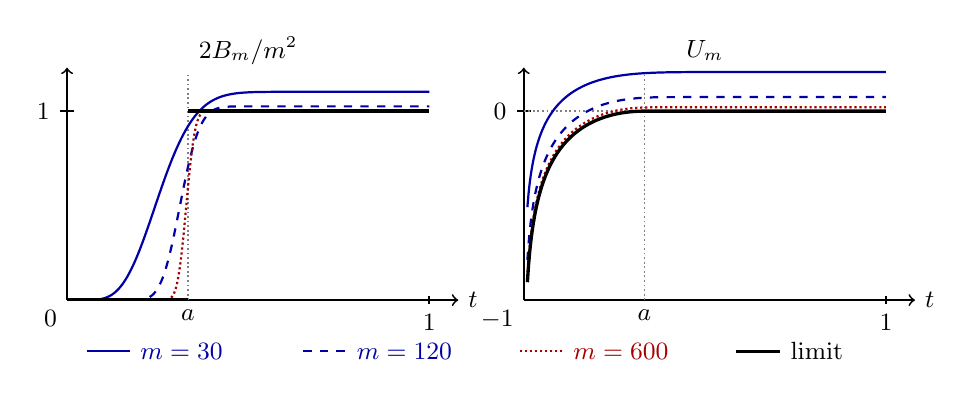
\begin{tikzpicture}[font=\small,line width=.65pt]
\begin{scope}[x=4.6cm,y=2.4cm]
\draw[->] (0,0)--(1.08,0) node[right] {$t$};
\draw[->] (0,0)--(0,1.23);
\node at (.5,1.32) {$2B_m/m^2$};
\node[below left] at (0,0) {$0$};
\draw (1,.02)--(1,-.02) node[below] {$1$};
\draw (.02,1)--(-.02,1) node[left] {$1$};
\draw[gray,densely dotted] (.333333,0)--(.333333,1.19);
\node[below] at (.333333,0) {$a$};
\begin{scope}\clip (0,0) rectangle (1,1.2);
\draw[blue!65!black,thick] plot coordinates {(0.000000,0.000000) (0.003333,0.000000) (0.006667,0.000000) (0.010000,0.000000) (0.013333,0.000000) (0.016667,0.000000) (0.020000,0.000000) (0.023333,0.000000) (0.026667,0.000001) (0.030000,0.000002) (0.033333,0.000005) (0.036667,0.000010) (0.040000,0.000019) (0.043333,0.000034) (0.046667,0.000057) (0.050000,0.000093) (0.053333,0.000146) (0.056667,0.000222) (0.060000,0.000328) (0.063333,0.000472) (0.066667,0.000665) (0.070000,0.000917) (0.073333,0.001243) (0.076667,0.001657) (0.080000,0.002175) (0.083333,0.002816) (0.086667,0.003598) (0.090000,0.004543) (0.093333,0.005672) (0.096667,0.007010) (0.100000,0.008579) (0.103333,0.010406) (0.106667,0.012516) (0.110000,0.014935) (0.113333,0.017689) (0.116667,0.020803) (0.120000,0.024304) (0.123333,0.028216) (0.126667,0.032564) (0.130000,0.037370) (0.133333,0.042656) (0.136667,0.048442) (0.140000,0.054746) (0.143333,0.061584) (0.146667,0.068971) (0.150000,0.076919) (0.153333,0.085436) (0.156667,0.094531) (0.160000,0.104207) (0.163333,0.114466) (0.166667,0.125308) (0.170000,0.136728) (0.173333,0.148721) (0.176667,0.161277) (0.180000,0.174384) (0.183333,0.188030) (0.186667,0.202196) (0.190000,0.216864) (0.193333,0.232014) (0.196667,0.247622) (0.200000,0.263662) (0.203333,0.280108) (0.206667,0.296932) (0.210000,0.314104) (0.213333,0.331593) (0.216667,0.349367) (0.220000,0.367393) (0.223333,0.385637) (0.226667,0.404066) (0.230000,0.422644) (0.233333,0.441339) (0.236667,0.460115) (0.240000,0.478939) (0.243333,0.497776) (0.246667,0.516594) (0.250000,0.535360) (0.253333,0.554044) (0.256667,0.572613) (0.260000,0.591040) (0.263333,0.609294) (0.266667,0.627351) (0.270000,0.645183) (0.273333,0.662766) (0.276667,0.680078) (0.280000,0.697098) (0.283333,0.713806) (0.286667,0.730183) (0.290000,0.746213) (0.293333,0.761882) (0.296667,0.777176) (0.300000,0.792083) (0.303333,0.806593) (0.306667,0.820698) (0.310000,0.834390) (0.313333,0.847664) (0.316667,0.860516) (0.320000,0.872943) (0.323333,0.884944) (0.326667,0.896518) (0.330000,0.907666) (0.333333,0.918390) (0.336667,0.928694) (0.340000,0.938582) (0.343333,0.948059) (0.346667,0.957130) (0.350000,0.965803) (0.353333,0.974084) (0.356667,0.981983) (0.360000,0.989507) (0.363333,0.996665) (0.366667,1.003469) (0.370000,1.009926) (0.373333,1.016048) (0.376667,1.021845) (0.380000,1.027329) (0.383333,1.032509) (0.386667,1.037397) (0.390000,1.042004) (0.393333,1.046341) (0.396667,1.050419) (0.400000,1.054249) (0.403333,1.057842) (0.406667,1.061209) (0.410000,1.064360) (0.413333,1.067306) (0.416667,1.070057) (0.420000,1.072622) (0.423333,1.075012) (0.426667,1.077236) (0.430000,1.079303) (0.433333,1.081221) (0.436667,1.083000) (0.440000,1.084648) (0.443333,1.086172) (0.446667,1.087580) (0.450000,1.088880) (0.453333,1.090078) (0.456667,1.091181) (0.460000,1.092195) (0.463333,1.093126) (0.466667,1.093981) (0.470000,1.094764) (0.473333,1.095480) (0.476667,1.096135) (0.480000,1.096733) (0.483333,1.097278) (0.486667,1.097774) (0.490000,1.098225) (0.493333,1.098635) (0.496667,1.099007) (0.500000,1.099344) (0.503333,1.099649) (0.506667,1.099924) (0.510000,1.100173) (0.513333,1.100397) (0.516667,1.100599) (0.520000,1.100780) (0.523333,1.100943) (0.526667,1.101089) (0.530000,1.101219) (0.533333,1.101336) (0.536667,1.101441) (0.540000,1.101534) (0.543333,1.101616) (0.546667,1.101690) (0.550000,1.101755) (0.553333,1.101813) (0.556667,1.101864) (0.560000,1.101910) (0.563333,1.101950) (0.566667,1.101985) (0.570000,1.102016) (0.573333,1.102043) (0.576667,1.102067) (0.580000,1.102088) (0.583333,1.102106) (0.586667,1.102122) (0.590000,1.102136) (0.593333,1.102148) (0.596667,1.102159) (0.600000,1.102168) (0.603333,1.102176) (0.606667,1.102183) (0.610000,1.102188) (0.613333,1.102193) (0.616667,1.102198) (0.620000,1.102202) (0.623333,1.102205) (0.626667,1.102207) (0.630000,1.102210) (0.633333,1.102212) (0.636667,1.102213) (0.640000,1.102215) (0.643333,1.102216) (0.646667,1.102217) (0.650000,1.102218) (0.653333,1.102219) (0.656667,1.102219) (0.660000,1.102220) (0.663333,1.102220) (0.666667,1.102221) (0.670000,1.102221) (0.673333,1.102221) (0.676667,1.102221) (0.680000,1.102221) (0.683333,1.102222) (0.686667,1.102222) (0.690000,1.102222) (0.693333,1.102222) (0.696667,1.102222) (0.700000,1.102222) (0.703333,1.102222) (0.706667,1.102222) (0.710000,1.102222) (0.713333,1.102222) (0.716667,1.102222) (0.720000,1.102222) (0.723333,1.102222) (0.726667,1.102222) (0.730000,1.102222) (0.733333,1.102222) (0.736667,1.102222) (0.740000,1.102222) (0.743333,1.102222) (0.746667,1.102222) (0.750000,1.102222) (0.753333,1.102222) (0.756667,1.102222) (0.760000,1.102222) (0.763333,1.102222) (0.766667,1.102222) (0.770000,1.102222) (0.773333,1.102222) (0.776667,1.102222) (0.780000,1.102222) (0.783333,1.102222) (0.786667,1.102222) (0.790000,1.102222) (0.793333,1.102222) (0.796667,1.102222) (0.800000,1.102222) (0.803333,1.102222) (0.806667,1.102222) (0.810000,1.102222) (0.813333,1.102222) (0.816667,1.102222) (0.820000,1.102222) (0.823333,1.102222) (0.826667,1.102222) (0.830000,1.102222) (0.833333,1.102222) (0.836667,1.102222) (0.840000,1.102222) (0.843333,1.102222) (0.846667,1.102222) (0.850000,1.102222) (0.853333,1.102222) (0.856667,1.102222) (0.860000,1.102222) (0.863333,1.102222) (0.866667,1.102222) (0.870000,1.102222) (0.873333,1.102222) (0.876667,1.102222) (0.880000,1.102222) (0.883333,1.102222) (0.886667,1.102222) (0.890000,1.102222) (0.893333,1.102222) (0.896667,1.102222) (0.900000,1.102222) (0.903333,1.102222) (0.906667,1.102222) (0.910000,1.102222) (0.913333,1.102222) (0.916667,1.102222) (0.920000,1.102222) (0.923333,1.102222) (0.926667,1.102222) (0.930000,1.102222) (0.933333,1.102222) (0.936667,1.102222) (0.940000,1.102222) (0.943333,1.102222) (0.946667,1.102222) (0.950000,1.102222) (0.953333,1.102222) (0.956667,1.102222) (0.960000,1.102222) (0.963333,1.102222) (0.966667,1.102222) (0.970000,1.102222) (0.973333,1.102222) (0.976667,1.102222) (0.980000,1.102222) (0.983333,1.102222) (0.986667,1.102222) (0.990000,1.102222) (0.993333,1.102222) (0.996667,1.102222) (1.000000,1.102222)};
\draw[blue!65!black,dashed,thick] plot coordinates {(0.000000,0.000000) (0.003333,0.000000) (0.006667,0.000000) (0.010000,0.000000) (0.013333,0.000000) (0.016667,0.000000) (0.020000,0.000000) (0.023333,0.000000) (0.026667,0.000000) (0.030000,0.000000) (0.033333,0.000000) (0.036667,0.000000) (0.040000,0.000000) (0.043333,0.000000) (0.046667,0.000000) (0.050000,0.000000) (0.053333,0.000000) (0.056667,0.000000) (0.060000,0.000000) (0.063333,0.000000) (0.066667,0.000000) (0.070000,0.000000) (0.073333,0.000000) (0.076667,0.000000) (0.080000,0.000000) (0.083333,0.000000) (0.086667,0.000000) (0.090000,0.000000) (0.093333,0.000000) (0.096667,0.000000) (0.100000,0.000000) (0.103333,0.000000) (0.106667,0.000000) (0.110000,0.000000) (0.113333,0.000000) (0.116667,0.000000) (0.120000,0.000000) (0.123333,0.000000) (0.126667,0.000000) (0.130000,0.000000) (0.133333,0.000000) (0.136667,0.000000) (0.140000,0.000001) (0.143333,0.000001) (0.146667,0.000002) (0.150000,0.000003) (0.153333,0.000006) (0.156667,0.000010) (0.160000,0.000016) (0.163333,0.000026) (0.166667,0.000041) (0.170000,0.000063) (0.173333,0.000096) (0.176667,0.000145) (0.180000,0.000215) (0.183333,0.000315) (0.186667,0.000454) (0.190000,0.000648) (0.193333,0.000912) (0.196667,0.001267) (0.200000,0.001741) (0.203333,0.002365) (0.206667,0.003176) (0.210000,0.004220) (0.213333,0.005549) (0.216667,0.007222) (0.220000,0.009308) (0.223333,0.011880) (0.226667,0.015023) (0.230000,0.018825) (0.233333,0.023383) (0.236667,0.028795) (0.240000,0.035165) (0.243333,0.042597) (0.246667,0.051193) (0.250000,0.061052) (0.253333,0.072266) (0.256667,0.084919) (0.260000,0.099083) (0.263333,0.114813) (0.266667,0.132150) (0.270000,0.151114) (0.273333,0.171706) (0.276667,0.193902) (0.280000,0.217657) (0.283333,0.242902) (0.286667,0.269544) (0.290000,0.297469) (0.293333,0.326543) (0.296667,0.356611) (0.300000,0.387506) (0.303333,0.419044) (0.306667,0.451035) (0.310000,0.483282) (0.313333,0.515583) (0.316667,0.547742) (0.320000,0.579564) (0.323333,0.610865) (0.326667,0.641470) (0.330000,0.671219) (0.333333,0.699967) (0.336667,0.727589) (0.340000,0.753977) (0.343333,0.779044) (0.346667,0.802722) (0.350000,0.824965) (0.353333,0.845743) (0.356667,0.865046) (0.360000,0.882883) (0.363333,0.899276) (0.366667,0.914260) (0.370000,0.927884) (0.373333,0.940205) (0.376667,0.951290) (0.380000,0.961210) (0.383333,0.970041) (0.386667,0.977863) (0.390000,0.984754) (0.393333,0.990794) (0.396667,0.996061) (0.400000,1.000631) (0.403333,1.004575) (0.406667,1.007963) (0.410000,1.010857) (0.413333,1.013317) (0.416667,1.015398) (0.420000,1.017150) (0.423333,1.018616) (0.426667,1.019838) (0.430000,1.020851) (0.433333,1.021686) (0.436667,1.022372) (0.440000,1.022931) (0.443333,1.023386) (0.446667,1.023754) (0.450000,1.024049) (0.453333,1.024286) (0.456667,1.024474) (0.460000,1.024624) (0.463333,1.024741) (0.466667,1.024833) (0.470000,1.024905) (0.473333,1.024961) (0.476667,1.025005) (0.480000,1.025038) (0.483333,1.025063) (0.486667,1.025082) (0.490000,1.025097) (0.493333,1.025108) (0.496667,1.025116) (0.500000,1.025122) (0.503333,1.025127) (0.506667,1.025130) (0.510000,1.025133) (0.513333,1.025134) (0.516667,1.025136) (0.520000,1.025137) (0.523333,1.025137) (0.526667,1.025138) (0.530000,1.025138) (0.533333,1.025138) (0.536667,1.025139) (0.540000,1.025139) (0.543333,1.025139) (0.546667,1.025139) (0.550000,1.025139) (0.553333,1.025139) (0.556667,1.025139) (0.560000,1.025139) (0.563333,1.025139) (0.566667,1.025139) (0.570000,1.025139) (0.573333,1.025139) (0.576667,1.025139) (0.580000,1.025139) (0.583333,1.025139) (0.586667,1.025139) (0.590000,1.025139) (0.593333,1.025139) (0.596667,1.025139) (0.600000,1.025139) (0.603333,1.025139) (0.606667,1.025139) (0.610000,1.025139) (0.613333,1.025139) (0.616667,1.025139) (0.620000,1.025139) (0.623333,1.025139) (0.626667,1.025139) (0.630000,1.025139) (0.633333,1.025139) (0.636667,1.025139) (0.640000,1.025139) (0.643333,1.025139) (0.646667,1.025139) (0.650000,1.025139) (0.653333,1.025139) (0.656667,1.025139) (0.660000,1.025139) (0.663333,1.025139) (0.666667,1.025139) (0.670000,1.025139) (0.673333,1.025139) (0.676667,1.025139) (0.680000,1.025139) (0.683333,1.025139) (0.686667,1.025139) (0.690000,1.025139) (0.693333,1.025139) (0.696667,1.025139) (0.700000,1.025139) (0.703333,1.025139) (0.706667,1.025139) (0.710000,1.025139) (0.713333,1.025139) (0.716667,1.025139) (0.720000,1.025139) (0.723333,1.025139) (0.726667,1.025139) (0.730000,1.025139) (0.733333,1.025139) (0.736667,1.025139) (0.740000,1.025139) (0.743333,1.025139) (0.746667,1.025139) (0.750000,1.025139) (0.753333,1.025139) (0.756667,1.025139) (0.760000,1.025139) (0.763333,1.025139) (0.766667,1.025139) (0.770000,1.025139) (0.773333,1.025139) (0.776667,1.025139) (0.780000,1.025139) (0.783333,1.025139) (0.786667,1.025139) (0.790000,1.025139) (0.793333,1.025139) (0.796667,1.025139) (0.800000,1.025139) (0.803333,1.025139) (0.806667,1.025139) (0.810000,1.025139) (0.813333,1.025139) (0.816667,1.025139) (0.820000,1.025139) (0.823333,1.025139) (0.826667,1.025139) (0.830000,1.025139) (0.833333,1.025139) (0.836667,1.025139) (0.840000,1.025139) (0.843333,1.025139) (0.846667,1.025139) (0.850000,1.025139) (0.853333,1.025139) (0.856667,1.025139) (0.860000,1.025139) (0.863333,1.025139) (0.866667,1.025139) (0.870000,1.025139) (0.873333,1.025139) (0.876667,1.025139) (0.880000,1.025139) (0.883333,1.025139) (0.886667,1.025139) (0.890000,1.025139) (0.893333,1.025139) (0.896667,1.025139) (0.900000,1.025139) (0.903333,1.025139) (0.906667,1.025139) (0.910000,1.025139) (0.913333,1.025139) (0.916667,1.025139) (0.920000,1.025139) (0.923333,1.025139) (0.926667,1.025139) (0.930000,1.025139) (0.933333,1.025139) (0.936667,1.025139) (0.940000,1.025139) (0.943333,1.025139) (0.946667,1.025139) (0.950000,1.025139) (0.953333,1.025139) (0.956667,1.025139) (0.960000,1.025139) (0.963333,1.025139) (0.966667,1.025139) (0.970000,1.025139) (0.973333,1.025139) (0.976667,1.025139) (0.980000,1.025139) (0.983333,1.025139) (0.986667,1.025139) (0.990000,1.025139) (0.993333,1.025139) (0.996667,1.025139) (1.000000,1.025139)};
\draw[red!65!black,densely dotted,thick] plot coordinates {(0.000000,0.000000) (0.003333,0.000000) (0.006667,0.000000) (0.010000,0.000000) (0.013333,0.000000) (0.016667,0.000000) (0.020000,0.000000) (0.023333,0.000000) (0.026667,0.000000) (0.030000,0.000000) (0.033333,0.000000) (0.036667,0.000000) (0.040000,0.000000) (0.043333,0.000000) (0.046667,0.000000) (0.050000,0.000000) (0.053333,0.000000) (0.056667,0.000000) (0.060000,0.000000) (0.063333,0.000000) (0.066667,0.000000) (0.070000,0.000000) (0.073333,0.000000) (0.076667,0.000000) (0.080000,0.000000) (0.083333,0.000000) (0.086667,0.000000) (0.090000,0.000000) (0.093333,0.000000) (0.096667,0.000000) (0.100000,0.000000) (0.103333,0.000000) (0.106667,0.000000) (0.110000,0.000000) (0.113333,0.000000) (0.116667,0.000000) (0.120000,0.000000) (0.123333,0.000000) (0.126667,0.000000) (0.130000,0.000000) (0.133333,0.000000) (0.136667,0.000000) (0.140000,0.000000) (0.143333,0.000000) (0.146667,0.000000) (0.150000,0.000000) (0.153333,0.000000) (0.156667,0.000000) (0.160000,0.000000) (0.163333,0.000000) (0.166667,0.000000) (0.170000,0.000000) (0.173333,0.000000) (0.176667,0.000000) (0.180000,0.000000) (0.183333,0.000000) (0.186667,0.000000) (0.190000,0.000000) (0.193333,0.000000) (0.196667,0.000000) (0.200000,0.000000) (0.203333,0.000000) (0.206667,0.000000) (0.210000,0.000000) (0.213333,0.000000) (0.216667,0.000000) (0.220000,0.000000) (0.223333,0.000000) (0.226667,0.000000) (0.230000,0.000000) (0.233333,0.000000) (0.236667,0.000000) (0.240000,0.000000) (0.243333,0.000001) (0.246667,0.000003) (0.250000,0.000007) (0.253333,0.000016) (0.256667,0.000037) (0.260000,0.000081) (0.263333,0.000171) (0.266667,0.000348) (0.270000,0.000681) (0.273333,0.001284) (0.276667,0.002337) (0.280000,0.004106) (0.283333,0.006973) (0.286667,0.011454) (0.290000,0.018212) (0.293333,0.028056) (0.296667,0.041907) (0.300000,0.060743) (0.303333,0.085513) (0.306667,0.117026) (0.310000,0.155828) (0.313333,0.202089) (0.316667,0.255512) (0.320000,0.315292) (0.323333,0.380137) (0.326667,0.448342) (0.330000,0.517931) (0.333333,0.586824) (0.336667,0.653023) (0.340000,0.714784) (0.343333,0.770742) (0.346667,0.819993) (0.350000,0.862114) (0.353333,0.897125) (0.356667,0.925415) (0.360000,0.947641) (0.363333,0.964625) (0.366667,0.977249) (0.370000,0.986378) (0.373333,0.992802) (0.376667,0.997202) (0.380000,1.000136) (0.383333,1.002039) (0.386667,1.003243) (0.390000,1.003983) (0.393333,1.004427) (0.396667,1.004686) (0.400000,1.004833) (0.403333,1.004915) (0.406667,1.004959) (0.410000,1.004982) (0.413333,1.004994) (0.416667,1.005000) (0.420000,1.005003) (0.423333,1.005004) (0.426667,1.005005) (0.430000,1.005005) (0.433333,1.005005) (0.436667,1.005006) (0.440000,1.005006) (0.443333,1.005006) (0.446667,1.005006) (0.450000,1.005006) (0.453333,1.005006) (0.456667,1.005006) (0.460000,1.005006) (0.463333,1.005006) (0.466667,1.005006) (0.470000,1.005006) (0.473333,1.005006) (0.476667,1.005006) (0.480000,1.005006) (0.483333,1.005006) (0.486667,1.005006) (0.490000,1.005006) (0.493333,1.005006) (0.496667,1.005006) (0.500000,1.005006) (0.503333,1.005006) (0.506667,1.005006) (0.510000,1.005006) (0.513333,1.005006) (0.516667,1.005006) (0.520000,1.005006) (0.523333,1.005006) (0.526667,1.005006) (0.530000,1.005006) (0.533333,1.005006) (0.536667,1.005006) (0.540000,1.005006) (0.543333,1.005006) (0.546667,1.005006) (0.550000,1.005006) (0.553333,1.005006) (0.556667,1.005006) (0.560000,1.005006) (0.563333,1.005006) (0.566667,1.005006) (0.570000,1.005006) (0.573333,1.005006) (0.576667,1.005006) (0.580000,1.005006) (0.583333,1.005006) (0.586667,1.005006) (0.590000,1.005006) (0.593333,1.005006) (0.596667,1.005006) (0.600000,1.005006) (0.603333,1.005006) (0.606667,1.005006) (0.610000,1.005006) (0.613333,1.005006) (0.616667,1.005006) (0.620000,1.005006) (0.623333,1.005006) (0.626667,1.005006) (0.630000,1.005006) (0.633333,1.005006) (0.636667,1.005006) (0.640000,1.005006) (0.643333,1.005006) (0.646667,1.005006) (0.650000,1.005006) (0.653333,1.005006) (0.656667,1.005006) (0.660000,1.005006) (0.663333,1.005006) (0.666667,1.005006) (0.670000,1.005006) (0.673333,1.005006) (0.676667,1.005006) (0.680000,1.005006) (0.683333,1.005006) (0.686667,1.005006) (0.690000,1.005006) (0.693333,1.005006) (0.696667,1.005006) (0.700000,1.005006) (0.703333,1.005006) (0.706667,1.005006) (0.710000,1.005006) (0.713333,1.005006) (0.716667,1.005006) (0.720000,1.005006) (0.723333,1.005006) (0.726667,1.005006) (0.730000,1.005006) (0.733333,1.005006) (0.736667,1.005006) (0.740000,1.005006) (0.743333,1.005006) (0.746667,1.005006) (0.750000,1.005006) (0.753333,1.005006) (0.756667,1.005006) (0.760000,1.005006) (0.763333,1.005006) (0.766667,1.005006) (0.770000,1.005006) (0.773333,1.005006) (0.776667,1.005006) (0.780000,1.005006) (0.783333,1.005006) (0.786667,1.005006) (0.790000,1.005006) (0.793333,1.005006) (0.796667,1.005006) (0.800000,1.005006) (0.803333,1.005006) (0.806667,1.005006) (0.810000,1.005006) (0.813333,1.005006) (0.816667,1.005006) (0.820000,1.005006) (0.823333,1.005006) (0.826667,1.005006) (0.830000,1.005006) (0.833333,1.005006) (0.836667,1.005006) (0.840000,1.005006) (0.843333,1.005006) (0.846667,1.005006) (0.850000,1.005006) (0.853333,1.005006) (0.856667,1.005006) (0.860000,1.005006) (0.863333,1.005006) (0.866667,1.005006) (0.870000,1.005006) (0.873333,1.005006) (0.876667,1.005006) (0.880000,1.005006) (0.883333,1.005006) (0.886667,1.005006) (0.890000,1.005006) (0.893333,1.005006) (0.896667,1.005006) (0.900000,1.005006) (0.903333,1.005006) (0.906667,1.005006) (0.910000,1.005006) (0.913333,1.005006) (0.916667,1.005006) (0.920000,1.005006) (0.923333,1.005006) (0.926667,1.005006) (0.930000,1.005006) (0.933333,1.005006) (0.936667,1.005006) (0.940000,1.005006) (0.943333,1.005006) (0.946667,1.005006) (0.950000,1.005006) (0.953333,1.005006) (0.956667,1.005006) (0.960000,1.005006) (0.963333,1.005006) (0.966667,1.005006) (0.970000,1.005006) (0.973333,1.005006) (0.976667,1.005006) (0.980000,1.005006) (0.983333,1.005006) (0.986667,1.005006) (0.990000,1.005006) (0.993333,1.005006) (0.996667,1.005006) (1.000000,1.005006)};
\draw[black,very thick] (0,0)--(.333333,0);
\draw[black,very thick] (.333333,1)--(1,1);
\end{scope}\end{scope}
\begin{scope}[xshift=5.8cm,x=4.6cm,y=2.4cm]
\draw[->] (0,0)--(1.08,0) node[right] {$t$};
\draw[->] (0,0)--(0,1.23);
\node at (.5,1.32) {$U_m$};
\node[below left] at (0,0) {$-1$};
\draw (1,.02)--(1,-.02) node[below] {$1$};
\draw (.02,1)--(-.02,1) node[left] {$0$};
\draw[gray,densely dotted] (0,1)--(1,1);
\draw[gray,densely dotted] (.333333,0)--(.333333,1.19);
\node[below] at (.333333,0) {$a$};
\begin{scope}\clip (0,0) rectangle (1,1.22);
\draw[blue!65!black,thick] plot coordinates {(0.010000,0.491716) (0.013300,0.565596) (0.016600,0.622527) (0.019900,0.668702) (0.023200,0.707436) (0.026500,0.740715) (0.029800,0.769821) (0.033100,0.795633) (0.036400,0.818776) (0.039700,0.839714) (0.043000,0.858799) (0.046300,0.876304) (0.049600,0.892446) (0.052900,0.907401) (0.056200,0.921311) (0.059500,0.934297) (0.062800,0.946456) (0.066100,0.957874) (0.069400,0.968621) (0.072700,0.978761) (0.076000,0.988347) (0.079300,0.997426) (0.082600,1.006038) (0.085900,1.014219) (0.089200,1.022003) (0.092500,1.029418) (0.095800,1.036489) (0.099100,1.043240) (0.102400,1.049691) (0.105700,1.055861) (0.109000,1.061767) (0.112300,1.067424) (0.115600,1.072848) (0.118900,1.078051) (0.122200,1.083045) (0.125500,1.087840) (0.128800,1.092448) (0.132100,1.096877) (0.135400,1.101137) (0.138700,1.105235) (0.142000,1.109178) (0.145300,1.112975) (0.148600,1.116631) (0.151900,1.120153) (0.155200,1.123546) (0.158500,1.126816) (0.161800,1.129967) (0.165100,1.133005) (0.168400,1.135934) (0.171700,1.138758) (0.175000,1.141482) (0.178300,1.144109) (0.181600,1.146642) (0.184900,1.149085) (0.188200,1.151442) (0.191500,1.153715) (0.194800,1.155908) (0.198100,1.158022) (0.201400,1.160061) (0.204700,1.162028) (0.208000,1.163924) (0.211300,1.165753) (0.214600,1.167516) (0.217900,1.169215) (0.221200,1.170853) (0.224500,1.172431) (0.227800,1.173951) (0.231100,1.175416) (0.234400,1.176827) (0.237700,1.178185) (0.241000,1.179493) (0.244300,1.180752) (0.247600,1.181963) (0.250900,1.183128) (0.254200,1.184248) (0.257500,1.185325) (0.260800,1.186360) (0.264100,1.187354) (0.267400,1.188309) (0.270700,1.189226) (0.274000,1.190105) (0.277300,1.190949) (0.280600,1.191759) (0.283900,1.192534) (0.287200,1.193278) (0.290500,1.193989) (0.293800,1.194671) (0.297100,1.195323) (0.300400,1.195946) (0.303700,1.196542) (0.307000,1.197111) (0.310300,1.197655) (0.313600,1.198174) (0.316900,1.198668) (0.320200,1.199140) (0.323500,1.199589) (0.326800,1.200017) (0.330100,1.200424) (0.333400,1.200811) (0.336700,1.201179) (0.340000,1.201529) (0.343300,1.201860) (0.346600,1.202175) (0.349900,1.202473) (0.353200,1.202755) (0.356500,1.203022) (0.359800,1.203275) (0.363100,1.203514) (0.366400,1.203739) (0.369700,1.203952) (0.373000,1.204153) (0.376300,1.204342) (0.379600,1.204519) (0.382900,1.204687) (0.386200,1.204844) (0.389500,1.204992) (0.392800,1.205130) (0.396100,1.205260) (0.399400,1.205381) (0.402700,1.205495) (0.406000,1.205601) (0.409300,1.205701) (0.412600,1.205793) (0.415900,1.205879) (0.419200,1.205960) (0.422500,1.206035) (0.425800,1.206104) (0.429100,1.206169) (0.432400,1.206229) (0.435700,1.206284) (0.439000,1.206335) (0.442300,1.206383) (0.445600,1.206427) (0.448900,1.206467) (0.452200,1.206504) (0.455500,1.206539) (0.458800,1.206570) (0.462100,1.206599) (0.465400,1.206626) (0.468700,1.206650) (0.472000,1.206673) (0.475300,1.206693) (0.478600,1.206712) (0.481900,1.206729) (0.485200,1.206745) (0.488500,1.206759) (0.491800,1.206772) (0.495100,1.206783) (0.498400,1.206794) (0.501700,1.206804) (0.505000,1.206812) (0.508300,1.206820) (0.511600,1.206827) (0.514900,1.206834) (0.518200,1.206839) (0.521500,1.206845) (0.524800,1.206849) (0.528100,1.206853) (0.531400,1.206857) (0.534700,1.206860) (0.538000,1.206863) (0.541300,1.206866) (0.544600,1.206868) (0.547900,1.206871) (0.551200,1.206872) (0.554500,1.206874) (0.557800,1.206876) (0.561100,1.206877) (0.564400,1.206878) (0.567700,1.206879) (0.571000,1.206880) (0.574300,1.206881) (0.577600,1.206881) (0.580900,1.206882) (0.584200,1.206882) (0.587500,1.206883) (0.590800,1.206883) (0.594100,1.206884) (0.597400,1.206884) (0.600700,1.206884) (0.604000,1.206885) (0.607300,1.206885) (0.610600,1.206885) (0.613900,1.206885) (0.617200,1.206885) (0.620500,1.206885) (0.623800,1.206885) (0.627100,1.206885) (0.630400,1.206885) (0.633700,1.206886) (0.637000,1.206886) (0.640300,1.206886) (0.643600,1.206886) (0.646900,1.206886) (0.650200,1.206886) (0.653500,1.206886) (0.656800,1.206886) (0.660100,1.206886) (0.663400,1.206886) (0.666700,1.206886) (0.670000,1.206886) (0.673300,1.206886) (0.676600,1.206886) (0.679900,1.206886) (0.683200,1.206886) (0.686500,1.206886) (0.689800,1.206886) (0.693100,1.206886) (0.696400,1.206886) (0.699700,1.206886) (0.703000,1.206886) (0.706300,1.206886) (0.709600,1.206886) (0.712900,1.206886) (0.716200,1.206886) (0.719500,1.206886) (0.722800,1.206886) (0.726100,1.206886) (0.729400,1.206886) (0.732700,1.206886) (0.736000,1.206886) (0.739300,1.206886) (0.742600,1.206886) (0.745900,1.206886) (0.749200,1.206886) (0.752500,1.206886) (0.755800,1.206886) (0.759100,1.206886) (0.762400,1.206886) (0.765700,1.206886) (0.769000,1.206886) (0.772300,1.206886) (0.775600,1.206886) (0.778900,1.206886) (0.782200,1.206886) (0.785500,1.206886) (0.788800,1.206886) (0.792100,1.206886) (0.795400,1.206886) (0.798700,1.206886) (0.802000,1.206886) (0.805300,1.206886) (0.808600,1.206886) (0.811900,1.206886) (0.815200,1.206886) (0.818500,1.206886) (0.821800,1.206886) (0.825100,1.206886) (0.828400,1.206886) (0.831700,1.206886) (0.835000,1.206886) (0.838300,1.206886) (0.841600,1.206886) (0.844900,1.206886) (0.848200,1.206886) (0.851500,1.206886) (0.854800,1.206886) (0.858100,1.206886) (0.861400,1.206886) (0.864700,1.206886) (0.868000,1.206886) (0.871300,1.206886) (0.874600,1.206886) (0.877900,1.206886) (0.881200,1.206886) (0.884500,1.206886) (0.887800,1.206886) (0.891100,1.206886) (0.894400,1.206886) (0.897700,1.206886) (0.901000,1.206886) (0.904300,1.206886) (0.907600,1.206886) (0.910900,1.206886) (0.914200,1.206886) (0.917500,1.206886) (0.920800,1.206886) (0.924100,1.206886) (0.927400,1.206886) (0.930700,1.206886) (0.934000,1.206886) (0.937300,1.206886) (0.940600,1.206886) (0.943900,1.206886) (0.947200,1.206886) (0.950500,1.206886) (0.953800,1.206886) (0.957100,1.206886) (0.960400,1.206886) (0.963700,1.206886) (0.967000,1.206886) (0.970300,1.206886) (0.973600,1.206886) (0.976900,1.206886) (0.980200,1.206886) (0.983500,1.206886) (0.986800,1.206886) (0.990100,1.206886) (0.993400,1.206886) (0.996700,1.206886) (1.000000,1.206886)};
\draw[blue!65!black,dashed,thick] plot coordinates {(0.010000,0.212312) (0.013300,0.300397) (0.016600,0.368355) (0.019900,0.423538) (0.023200,0.469883) (0.026500,0.509749) (0.029800,0.544658) (0.033100,0.575654) (0.036400,0.603479) (0.039700,0.628684) (0.043000,0.651685) (0.046300,0.672810) (0.049600,0.692314) (0.052900,0.710406) (0.056200,0.727256) (0.059500,0.743006) (0.062800,0.757772) (0.066100,0.771655) (0.069400,0.784741) (0.072700,0.797103) (0.076000,0.808804) (0.079300,0.819900) (0.082600,0.830440) (0.085900,0.840466) (0.089200,0.850017) (0.092500,0.859127) (0.095800,0.867826) (0.099100,0.876142) (0.102400,0.884098) (0.105700,0.891718) (0.109000,0.899021) (0.112300,0.906026) (0.115600,0.912750) (0.118900,0.919208) (0.122200,0.925414) (0.125500,0.931381) (0.128800,0.937122) (0.132100,0.942646) (0.135400,0.947965) (0.138700,0.953088) (0.142000,0.958024) (0.145300,0.962781) (0.148600,0.967366) (0.151900,0.971788) (0.155200,0.976052) (0.158500,0.980165) (0.161800,0.984133) (0.165100,0.987961) (0.168400,0.991654) (0.171700,0.995218) (0.175000,0.998657) (0.178300,1.001976) (0.181600,1.005178) (0.184900,1.008268) (0.188200,1.011249) (0.191500,1.014125) (0.194800,1.016899) (0.198100,1.019575) (0.201400,1.022155) (0.204700,1.024642) (0.208000,1.027040) (0.211300,1.029350) (0.214600,1.031576) (0.217900,1.033719) (0.221200,1.035782) (0.224500,1.037768) (0.227800,1.039678) (0.231100,1.041515) (0.234400,1.043280) (0.237700,1.044976) (0.241000,1.046604) (0.244300,1.048166) (0.247600,1.049665) (0.250900,1.051101) (0.254200,1.052476) (0.257500,1.053792) (0.260800,1.055050) (0.264100,1.056253) (0.267400,1.057401) (0.270700,1.058496) (0.274000,1.059539) (0.277300,1.060532) (0.280600,1.061477) (0.283900,1.062374) (0.287200,1.063225) (0.290500,1.064031) (0.293800,1.064794) (0.297100,1.065515) (0.300400,1.066195) (0.303700,1.066836) (0.307000,1.067439) (0.310300,1.068006) (0.313600,1.068536) (0.316900,1.069033) (0.320200,1.069497) (0.323500,1.069929) (0.326800,1.070331) (0.330100,1.070704) (0.333400,1.071049) (0.336700,1.071368) (0.340000,1.071662) (0.343300,1.071932) (0.346600,1.072179) (0.349900,1.072405) (0.353200,1.072611) (0.356500,1.072798) (0.359800,1.072968) (0.363100,1.073120) (0.366400,1.073258) (0.369700,1.073381) (0.373000,1.073491) (0.376300,1.073589) (0.379600,1.073676) (0.382900,1.073752) (0.386200,1.073820) (0.389500,1.073879) (0.392800,1.073931) (0.396100,1.073975) (0.399400,1.074014) (0.402700,1.074047) (0.406000,1.074076) (0.409300,1.074101) (0.412600,1.074121) (0.415900,1.074139) (0.419200,1.074154) (0.422500,1.074166) (0.425800,1.074177) (0.429100,1.074185) (0.432400,1.074192) (0.435700,1.074198) (0.439000,1.074203) (0.442300,1.074207) (0.445600,1.074210) (0.448900,1.074213) (0.452200,1.074215) (0.455500,1.074216) (0.458800,1.074218) (0.462100,1.074219) (0.465400,1.074219) (0.468700,1.074220) (0.472000,1.074221) (0.475300,1.074221) (0.478600,1.074221) (0.481900,1.074222) (0.485200,1.074222) (0.488500,1.074222) (0.491800,1.074222) (0.495100,1.074222) (0.498400,1.074222) (0.501700,1.074222) (0.505000,1.074222) (0.508300,1.074222) (0.511600,1.074222) (0.514900,1.074222) (0.518200,1.074222) (0.521500,1.074222) (0.524800,1.074222) (0.528100,1.074222) (0.531400,1.074222) (0.534700,1.074222) (0.538000,1.074222) (0.541300,1.074222) (0.544600,1.074222) (0.547900,1.074222) (0.551200,1.074222) (0.554500,1.074222) (0.557800,1.074222) (0.561100,1.074222) (0.564400,1.074222) (0.567700,1.074222) (0.571000,1.074222) (0.574300,1.074222) (0.577600,1.074222) (0.580900,1.074222) (0.584200,1.074222) (0.587500,1.074222) (0.590800,1.074222) (0.594100,1.074222) (0.597400,1.074222) (0.600700,1.074222) (0.604000,1.074222) (0.607300,1.074222) (0.610600,1.074222) (0.613900,1.074222) (0.617200,1.074222) (0.620500,1.074222) (0.623800,1.074222) (0.627100,1.074222) (0.630400,1.074222) (0.633700,1.074222) (0.637000,1.074222) (0.640300,1.074222) (0.643600,1.074222) (0.646900,1.074222) (0.650200,1.074222) (0.653500,1.074222) (0.656800,1.074222) (0.660100,1.074222) (0.663400,1.074222) (0.666700,1.074222) (0.670000,1.074222) (0.673300,1.074222) (0.676600,1.074222) (0.679900,1.074222) (0.683200,1.074222) (0.686500,1.074222) (0.689800,1.074222) (0.693100,1.074222) (0.696400,1.074222) (0.699700,1.074222) (0.703000,1.074222) (0.706300,1.074222) (0.709600,1.074222) (0.712900,1.074222) (0.716200,1.074222) (0.719500,1.074222) (0.722800,1.074222) (0.726100,1.074222) (0.729400,1.074222) (0.732700,1.074222) (0.736000,1.074222) (0.739300,1.074222) (0.742600,1.074222) (0.745900,1.074222) (0.749200,1.074222) (0.752500,1.074222) (0.755800,1.074222) (0.759100,1.074222) (0.762400,1.074222) (0.765700,1.074222) (0.769000,1.074222) (0.772300,1.074222) (0.775600,1.074222) (0.778900,1.074222) (0.782200,1.074222) (0.785500,1.074222) (0.788800,1.074222) (0.792100,1.074222) (0.795400,1.074222) (0.798700,1.074222) (0.802000,1.074222) (0.805300,1.074222) (0.808600,1.074222) (0.811900,1.074222) (0.815200,1.074222) (0.818500,1.074222) (0.821800,1.074222) (0.825100,1.074222) (0.828400,1.074222) (0.831700,1.074222) (0.835000,1.074222) (0.838300,1.074222) (0.841600,1.074222) (0.844900,1.074222) (0.848200,1.074222) (0.851500,1.074222) (0.854800,1.074222) (0.858100,1.074222) (0.861400,1.074222) (0.864700,1.074222) (0.868000,1.074222) (0.871300,1.074222) (0.874600,1.074222) (0.877900,1.074222) (0.881200,1.074222) (0.884500,1.074222) (0.887800,1.074222) (0.891100,1.074222) (0.894400,1.074222) (0.897700,1.074222) (0.901000,1.074222) (0.904300,1.074222) (0.907600,1.074222) (0.910900,1.074222) (0.914200,1.074222) (0.917500,1.074222) (0.920800,1.074222) (0.924100,1.074222) (0.927400,1.074222) (0.930700,1.074222) (0.934000,1.074222) (0.937300,1.074222) (0.940600,1.074222) (0.943900,1.074222) (0.947200,1.074222) (0.950500,1.074222) (0.953800,1.074222) (0.957100,1.074222) (0.960400,1.074222) (0.963700,1.074222) (0.967000,1.074222) (0.970300,1.074222) (0.973600,1.074222) (0.976900,1.074222) (0.980200,1.074222) (0.983500,1.074222) (0.986800,1.074222) (0.990100,1.074222) (0.993400,1.074222) (0.996700,1.074222) (1.000000,1.074222)};
\draw[red!65!black,densely dotted,thick] plot coordinates {(0.010000,0.122344) (0.013300,0.214227) (0.016600,0.285135) (0.019900,0.342730) (0.023200,0.391115) (0.026500,0.432748) (0.029800,0.469215) (0.033100,0.501603) (0.036400,0.530687) (0.039700,0.557040) (0.043000,0.581097) (0.046300,0.603197) (0.049600,0.623608) (0.052900,0.642548) (0.056200,0.660192) (0.059500,0.676690) (0.062800,0.692162) (0.066100,0.706714) (0.069400,0.720434) (0.072700,0.733399) (0.076000,0.745675) (0.079300,0.757321) (0.082600,0.768385) (0.085900,0.778915) (0.089200,0.788948) (0.092500,0.798521) (0.095800,0.807665) (0.099100,0.816409) (0.102400,0.824778) (0.105700,0.832795) (0.109000,0.840481) (0.112300,0.847856) (0.115600,0.854938) (0.118900,0.861741) (0.122200,0.868281) (0.125500,0.874570) (0.128800,0.880623) (0.132100,0.886450) (0.135400,0.892061) (0.138700,0.897467) (0.142000,0.902677) (0.145300,0.907699) (0.148600,0.912541) (0.151900,0.917211) (0.155200,0.921716) (0.158500,0.926061) (0.161800,0.930254) (0.165100,0.934299) (0.168400,0.938203) (0.171700,0.941971) (0.175000,0.945606) (0.178300,0.949114) (0.181600,0.952499) (0.184900,0.955764) (0.188200,0.958914) (0.191500,0.961953) (0.194800,0.964883) (0.198100,0.967708) (0.201400,0.970431) (0.204700,0.973055) (0.208000,0.975583) (0.211300,0.978017) (0.214600,0.980360) (0.217900,0.982614) (0.221200,0.984782) (0.224500,0.986865) (0.227800,0.988867) (0.231100,0.990788) (0.234400,0.992631) (0.237700,0.994399) (0.241000,0.996091) (0.244300,0.997711) (0.247600,0.999260) (0.250900,1.000739) (0.254200,1.002151) (0.257500,1.003496) (0.260800,1.004776) (0.264100,1.005993) (0.267400,1.007148) (0.270700,1.008241) (0.274000,1.009276) (0.277300,1.010252) (0.280600,1.011172) (0.283900,1.012036) (0.287200,1.012846) (0.290500,1.013603) (0.293800,1.014309) (0.297100,1.014964) (0.300400,1.015570) (0.303700,1.016129) (0.307000,1.016642) (0.310300,1.017110) (0.313600,1.017536) (0.316900,1.017920) (0.320200,1.018264) (0.323500,1.018570) (0.326800,1.018841) (0.330100,1.019078) (0.333400,1.019283) (0.336700,1.019459) (0.340000,1.019608) (0.343300,1.019733) (0.346600,1.019835) (0.349900,1.019918) (0.353200,1.019985) (0.356500,1.020036) (0.359800,1.020076) (0.363100,1.020106) (0.366400,1.020128) (0.369700,1.020144) (0.373000,1.020155) (0.376300,1.020163) (0.379600,1.020168) (0.382900,1.020171) (0.386200,1.020173) (0.389500,1.020174) (0.392800,1.020175) (0.396100,1.020176) (0.399400,1.020176) (0.402700,1.020176) (0.406000,1.020176) (0.409300,1.020176) (0.412600,1.020176) (0.415900,1.020176) (0.419200,1.020176) (0.422500,1.020176) (0.425800,1.020176) (0.429100,1.020176) (0.432400,1.020176) (0.435700,1.020176) (0.439000,1.020176) (0.442300,1.020176) (0.445600,1.020176) (0.448900,1.020176) (0.452200,1.020176) (0.455500,1.020176) (0.458800,1.020176) (0.462100,1.020176) (0.465400,1.020176) (0.468700,1.020176) (0.472000,1.020176) (0.475300,1.020176) (0.478600,1.020176) (0.481900,1.020176) (0.485200,1.020176) (0.488500,1.020176) (0.491800,1.020176) (0.495100,1.020176) (0.498400,1.020176) (0.501700,1.020176) (0.505000,1.020176) (0.508300,1.020176) (0.511600,1.020176) (0.514900,1.020176) (0.518200,1.020176) (0.521500,1.020176) (0.524800,1.020176) (0.528100,1.020176) (0.531400,1.020176) (0.534700,1.020176) (0.538000,1.020176) (0.541300,1.020176) (0.544600,1.020176) (0.547900,1.020176) (0.551200,1.020176) (0.554500,1.020176) (0.557800,1.020176) (0.561100,1.020176) (0.564400,1.020176) (0.567700,1.020176) (0.571000,1.020176) (0.574300,1.020176) (0.577600,1.020176) (0.580900,1.020176) (0.584200,1.020176) (0.587500,1.020176) (0.590800,1.020176) (0.594100,1.020176) (0.597400,1.020176) (0.600700,1.020176) (0.604000,1.020176) (0.607300,1.020176) (0.610600,1.020176) (0.613900,1.020176) (0.617200,1.020176) (0.620500,1.020176) (0.623800,1.020176) (0.627100,1.020176) (0.630400,1.020176) (0.633700,1.020176) (0.637000,1.020176) (0.640300,1.020176) (0.643600,1.020176) (0.646900,1.020176) (0.650200,1.020176) (0.653500,1.020176) (0.656800,1.020176) (0.660100,1.020176) (0.663400,1.020176) (0.666700,1.020176) (0.670000,1.020176) (0.673300,1.020176) (0.676600,1.020176) (0.679900,1.020176) (0.683200,1.020176) (0.686500,1.020176) (0.689800,1.020176) (0.693100,1.020176) (0.696400,1.020176) (0.699700,1.020176) (0.703000,1.020176) (0.706300,1.020176) (0.709600,1.020176) (0.712900,1.020176) (0.716200,1.020176) (0.719500,1.020176) (0.722800,1.020176) (0.726100,1.020176) (0.729400,1.020176) (0.732700,1.020176) (0.736000,1.020176) (0.739300,1.020176) (0.742600,1.020176) (0.745900,1.020176) (0.749200,1.020176) (0.752500,1.020176) (0.755800,1.020176) (0.759100,1.020176) (0.762400,1.020176) (0.765700,1.020176) (0.769000,1.020176) (0.772300,1.020176) (0.775600,1.020176) (0.778900,1.020176) (0.782200,1.020176) (0.785500,1.020176) (0.788800,1.020176) (0.792100,1.020176) (0.795400,1.020176) (0.798700,1.020176) (0.802000,1.020176) (0.805300,1.020176) (0.808600,1.020176) (0.811900,1.020176) (0.815200,1.020176) (0.818500,1.020176) (0.821800,1.020176) (0.825100,1.020176) (0.828400,1.020176) (0.831700,1.020176) (0.835000,1.020176) (0.838300,1.020176) (0.841600,1.020176) (0.844900,1.020176) (0.848200,1.020176) (0.851500,1.020176) (0.854800,1.020176) (0.858100,1.020176) (0.861400,1.020176) (0.864700,1.020176) (0.868000,1.020176) (0.871300,1.020176) (0.874600,1.020176) (0.877900,1.020176) (0.881200,1.020176) (0.884500,1.020176) (0.887800,1.020176) (0.891100,1.020176) (0.894400,1.020176) (0.897700,1.020176) (0.901000,1.020176) (0.904300,1.020176) (0.907600,1.020176) (0.910900,1.020176) (0.914200,1.020176) (0.917500,1.020176) (0.920800,1.020176) (0.924100,1.020176) (0.927400,1.020176) (0.930700,1.020176) (0.934000,1.020176) (0.937300,1.020176) (0.940600,1.020176) (0.943900,1.020176) (0.947200,1.020176) (0.950500,1.020176) (0.953800,1.020176) (0.957100,1.020176) (0.960400,1.020176) (0.963700,1.020176) (0.967000,1.020176) (0.970300,1.020176) (0.973600,1.020176) (0.976900,1.020176) (0.980200,1.020176) (0.983500,1.020176) (0.986800,1.020176) (0.990100,1.020176) (0.993400,1.020176) (0.996700,1.020176) (1.000000,1.020176)};
\draw[black,very thick] plot coordinates {(0.010000,0.094757) (0.013300,0.187591) (0.016600,0.259237) (0.019900,0.317435) (0.023200,0.366331) (0.026500,0.408406) (0.029800,0.445263) (0.033100,0.478000) (0.036400,0.507399) (0.039700,0.534040) (0.043000,0.558361) (0.046300,0.580706) (0.049600,0.601344) (0.052900,0.620496) (0.056200,0.638341) (0.059500,0.655025) (0.062800,0.670675) (0.066100,0.685395) (0.069400,0.699274) (0.072700,0.712391) (0.076000,0.724811) (0.079300,0.736594) (0.082600,0.747791) (0.085900,0.758447) (0.089200,0.768601) (0.092500,0.778291) (0.095800,0.787547) (0.099100,0.796398) (0.102400,0.804871) (0.105700,0.812988) (0.109000,0.820771) (0.112300,0.828239) (0.115600,0.835411) (0.118900,0.842301) (0.122200,0.848924) (0.125500,0.855296) (0.128800,0.861427) (0.132100,0.867330) (0.135400,0.873015) (0.138700,0.878492) (0.142000,0.883771) (0.145300,0.888859) (0.148600,0.893766) (0.151900,0.898499) (0.155200,0.903064) (0.158500,0.907468) (0.161800,0.911717) (0.165100,0.915817) (0.168400,0.919774) (0.171700,0.923592) (0.175000,0.927276) (0.178300,0.930832) (0.181600,0.934262) (0.184900,0.937571) (0.188200,0.940763) (0.191500,0.943842) (0.194800,0.946810) (0.198100,0.949672) (0.201400,0.952430) (0.204700,0.955087) (0.208000,0.957646) (0.211300,0.960109) (0.214600,0.962480) (0.217900,0.964759) (0.221200,0.966951) (0.224500,0.969056) (0.227800,0.971077) (0.231100,0.973016) (0.234400,0.974875) (0.237700,0.976655) (0.241000,0.978359) (0.244300,0.979988) (0.247600,0.981542) (0.250900,0.983025) (0.254200,0.984438) (0.257500,0.985781) (0.260800,0.987056) (0.264100,0.988264) (0.267400,0.989407) (0.270700,0.990486) (0.274000,0.991502) (0.277300,0.992455) (0.280600,0.993347) (0.283900,0.994179) (0.287200,0.994952) (0.290500,0.995667) (0.293800,0.996324) (0.297100,0.996925) (0.300400,0.997470) (0.303700,0.997959) (0.307000,0.998395) (0.310300,0.998777) (0.313600,0.999105) (0.316900,0.999382) (0.320200,0.999607) (0.323500,0.999780) (0.326800,0.999903) (0.330100,0.999976) (0.333400,1.000000) (0.336700,1.000000) (0.340000,1.000000) (0.343300,1.000000) (0.346600,1.000000) (0.349900,1.000000) (0.353200,1.000000) (0.356500,1.000000) (0.359800,1.000000) (0.363100,1.000000) (0.366400,1.000000) (0.369700,1.000000) (0.373000,1.000000) (0.376300,1.000000) (0.379600,1.000000) (0.382900,1.000000) (0.386200,1.000000) (0.389500,1.000000) (0.392800,1.000000) (0.396100,1.000000) (0.399400,1.000000) (0.402700,1.000000) (0.406000,1.000000) (0.409300,1.000000) (0.412600,1.000000) (0.415900,1.000000) (0.419200,1.000000) (0.422500,1.000000) (0.425800,1.000000) (0.429100,1.000000) (0.432400,1.000000) (0.435700,1.000000) (0.439000,1.000000) (0.442300,1.000000) (0.445600,1.000000) (0.448900,1.000000) (0.452200,1.000000) (0.455500,1.000000) (0.458800,1.000000) (0.462100,1.000000) (0.465400,1.000000) (0.468700,1.000000) (0.472000,1.000000) (0.475300,1.000000) (0.478600,1.000000) (0.481900,1.000000) (0.485200,1.000000) (0.488500,1.000000) (0.491800,1.000000) (0.495100,1.000000) (0.498400,1.000000) (0.501700,1.000000) (0.505000,1.000000) (0.508300,1.000000) (0.511600,1.000000) (0.514900,1.000000) (0.518200,1.000000) (0.521500,1.000000) (0.524800,1.000000) (0.528100,1.000000) (0.531400,1.000000) (0.534700,1.000000) (0.538000,1.000000) (0.541300,1.000000) (0.544600,1.000000) (0.547900,1.000000) (0.551200,1.000000) (0.554500,1.000000) (0.557800,1.000000) (0.561100,1.000000) (0.564400,1.000000) (0.567700,1.000000) (0.571000,1.000000) (0.574300,1.000000) (0.577600,1.000000) (0.580900,1.000000) (0.584200,1.000000) (0.587500,1.000000) (0.590800,1.000000) (0.594100,1.000000) (0.597400,1.000000) (0.600700,1.000000) (0.604000,1.000000) (0.607300,1.000000) (0.610600,1.000000) (0.613900,1.000000) (0.617200,1.000000) (0.620500,1.000000) (0.623800,1.000000) (0.627100,1.000000) (0.630400,1.000000) (0.633700,1.000000) (0.637000,1.000000) (0.640300,1.000000) (0.643600,1.000000) (0.646900,1.000000) (0.650200,1.000000) (0.653500,1.000000) (0.656800,1.000000) (0.660100,1.000000) (0.663400,1.000000) (0.666700,1.000000) (0.670000,1.000000) (0.673300,1.000000) (0.676600,1.000000) (0.679900,1.000000) (0.683200,1.000000) (0.686500,1.000000) (0.689800,1.000000) (0.693100,1.000000) (0.696400,1.000000) (0.699700,1.000000) (0.703000,1.000000) (0.706300,1.000000) (0.709600,1.000000) (0.712900,1.000000) (0.716200,1.000000) (0.719500,1.000000) (0.722800,1.000000) (0.726100,1.000000) (0.729400,1.000000) (0.732700,1.000000) (0.736000,1.000000) (0.739300,1.000000) (0.742600,1.000000) (0.745900,1.000000) (0.749200,1.000000) (0.752500,1.000000) (0.755800,1.000000) (0.759100,1.000000) (0.762400,1.000000) (0.765700,1.000000) (0.769000,1.000000) (0.772300,1.000000) (0.775600,1.000000) (0.778900,1.000000) (0.782200,1.000000) (0.785500,1.000000) (0.788800,1.000000) (0.792100,1.000000) (0.795400,1.000000) (0.798700,1.000000) (0.802000,1.000000) (0.805300,1.000000) (0.808600,1.000000) (0.811900,1.000000) (0.815200,1.000000) (0.818500,1.000000) (0.821800,1.000000) (0.825100,1.000000) (0.828400,1.000000) (0.831700,1.000000) (0.835000,1.000000) (0.838300,1.000000) (0.841600,1.000000) (0.844900,1.000000) (0.848200,1.000000) (0.851500,1.000000) (0.854800,1.000000) (0.858100,1.000000) (0.861400,1.000000) (0.864700,1.000000) (0.868000,1.000000) (0.871300,1.000000) (0.874600,1.000000) (0.877900,1.000000) (0.881200,1.000000) (0.884500,1.000000) (0.887800,1.000000) (0.891100,1.000000) (0.894400,1.000000) (0.897700,1.000000) (0.901000,1.000000) (0.904300,1.000000) (0.907600,1.000000) (0.910900,1.000000) (0.914200,1.000000) (0.917500,1.000000) (0.920800,1.000000) (0.924100,1.000000) (0.927400,1.000000) (0.930700,1.000000) (0.934000,1.000000) (0.937300,1.000000) (0.940600,1.000000) (0.943900,1.000000) (0.947200,1.000000) (0.950500,1.000000) (0.953800,1.000000) (0.957100,1.000000) (0.960400,1.000000) (0.963700,1.000000) (0.967000,1.000000) (0.970300,1.000000) (0.973600,1.000000) (0.976900,1.000000) (0.980200,1.000000) (0.983500,1.000000) (0.986800,1.000000) (0.990100,1.000000) (0.993400,1.000000) (0.996700,1.000000) (1.000000,1.000000)};
\end{scope}\end{scope}
\draw[blue!65!black,thick] (0.25,-.65)--(0.8,-.65) node[right] {$m=30$};
\draw[blue!65!black,dashed,thick] (3.0,-.65)--(3.55,-.65) node[right] {$m=120$};
\draw[red!65!black,densely dotted,thick] (5.75,-.65)--(6.3,-.65) node[right] {$m=600$};
\draw[black,very thick] (8.5,-.65)--(9.05,-.65) node[right] {limit};
\end{tikzpicture}
}
\caption{The one-point model with $q=2$ and $a=1/3$. The normalized kernel density (left) and the Fubini--Study potential (right) are plotted against $t$. The black curves are their limits. The potential panel omits $t<0.01$, where the limit tends to $-\infty$.}
\label{fig:hopf-point-kernel-limit}
\end{figure}

The formula for $E_a$ has an intrinsic envelope interpretation. Set $\psi_a=a\log t$ on $\mathbb P^q$. This is $\sigma$-plurisubharmonic for $0<a<1$: away from $b$, its curvature is the convex combination of $\sigma$ and the semipositive form induced by the projection $[Z_0:Z']\mapsto[Z']$. For $q=1$, the second form is zero. The local logarithmic expression gives the positive extension at $b$.

\Needspace{16\baselineskip}
\begin{proposition}\label{prop:hopf-point-envelope}
The function $E_a$ belongs to $\PSH(\mathbb P^q,\sigma)$ and
\[
 E_a=E_{\sigma,\mathbb P^q}[\psi_a]_{\mathcal I}(0),
 \qquad
 \mathrm{MA}_\sigma(E_a)=\mathbf1_{\{t>a\}}\sigma^q.
\]
Moreover, $E_a\circ\pi$ is the largest $u\in\PSH(X_n,\alpha)$ satisfying $u\leq0$ and $u\preceq_{\mathcal I}\varphi$. Thus
\[
 \mathbf1_{\{t\circ\pi>a\}}\nu_X
       =\frac1{2n}\mathrm{MA}^{\mathrm{ext}}_\omega(E_a\circ\pi).
\]
\end{proposition}
\begin{proof}
In the chart $Z_0=1$, write $z=Z'/Z_0$ and $R^2=a/(1-a)$. For $|z|<R$, the local potential of $\sigma+\ddc E_a$ is
\[
 \log(1+|z|^2)+E_a
       =a\log|z|^2-a\log a-(1-a)\log(1-a).
\]
Its complex Hessian is positive and has rank $q-1$ away from zero. For $|z|>R$, the form is $\sigma$. The two expressions for $E_a$ have equal values and equal first derivatives at $|z|=R$. They therefore glue as a $C^{1,1}$ function near the interface, with no hypersurface term in its distributional Hessian. Near $b$ it has the logarithmic pole of coefficient $a$. This proves global $\sigma$-plurisubharmonicity and $E_a\simeq\psi_a$.

To verify the envelope bound, let $w\in\PSH(\mathbb P^q,\sigma)$ satisfy $w\leq0$ and $w\preceq_{\mathcal I}\psi_a$. By \cref{lem:analytic-ideal-dominance}, $w\leq\psi_a+C$. Fix a complex line through zero in the affine chart. If the restriction of $w+\log(1+|z|^2)$ is identically $-\infty$, there is nothing to prove on that line. Otherwise it is subharmonic. On its punctured disk of radius $R$, subtract $a\log|z|^2$. The result is subharmonic and bounded above near zero by the ordinary singularity inequality, so it extends subharmonically across zero. On the boundary its value is at most $\log(1+R^2)-a\log R^2$. The maximum principle gives exactly $w\leq E_a$ in the disk. Every point with $|z|<R$ lies on such a line; outside this ball $w\leq0=E_a$. Since $E_a$ itself is an admissible competitor, it is the stated envelope. Continuous zero obstacles make the quasi-everywhere and everywhere inequalities equivalent, as proved earlier.

On the complement of $b$, the local potentials are $C^{1,1}$. Their Bedford--Taylor top products are the almost-everywhere determinants of their complex Hessians: local convolution gives uniformly bounded Hessians converging almost everywhere, and dominated convergence identifies the determinant limit with the locally uniform Bedford--Taylor limit. The rank computation makes this determinant zero for $t<a$ and equal to $\sigma^q$ for $t>a$. The interface has smooth volume zero, and a $C^{1,1}$ local potential adds no measure there. The non-pluripolar measure gives $b$ zero mass. This proves the measure formula.

For the assertion on $X_n$, every $\alpha$-plurisubharmonic function is $u=w\circ\pi$ by \cref{prop:psh-descent-submersion}. Since $\varphi$ has analytic singularities, $u\preceq_{\mathcal I}\varphi$ implies $u\preceq\varphi$ by \cref{lem:analytic-ideal-dominance}. In product coordinates $(z,\tau)$ at $p$, restrict this inequality to $\tau=0$. It yields $w(z)\leq a\log|z|^2+C$, and hence $w\preceq\psi_a$ globally. Conversely, $w\preceq\psi_a$ gives
\[
 w(z)\leq a\log|z|^2+C
             \leq a\log(|z|^2+|\tau|^2)+C
\]
near $p$. Away from $p$, local boundedness of $\varphi$ and compactness make the upper inequality global. Thus $w\circ\pi\preceq\varphi$, which implies the ideal order. Applying analytic ideal domination on the base as well shows that the two ideal-constrained competitor families are exactly those already considered. Their largest members therefore agree under pullback. Finally \cref{thm:hopf-descended-hermitian-ma} and the base measure formula give the last identity.
\end{proof}

For sufficiently small rational $a$, the cutoff construction in the preceding section makes $\varphi\in\PSH(X_n,\omega)$ with its only pole at $p$. The theorem consequently applies on the Hopf threefold where BMP fails, and gives a nonzero limit with the intrinsic normalization $2/m^2$. The limiting potential has a pole on the whole elliptic fiber over $b$. At other points of that fiber the input $\varphi$ is locally bounded, whereas the limiting potential has a nontrivial multiplier ideal at sufficiently large weight. Thus even this positive-growth limit does not recover the multiplier-ideal type of an arbitrary Hermitian-positive selecting weight.

\enlargethispage{2\baselineskip}
The measure limit is also different from the raw Hermitian Monge--Amp\`ere measure of $\varphi$. Choose its cutoff support in a small neighborhood of $p$. There is a nonempty open set outside that support with $t\circ\pi<a$: take a neighborhood of another point of the same elliptic fiber. On this open set $\varphi=0$, so locality gives $\mathrm{MA}^{\mathrm{ext}}_\omega(\varphi)=\omega^n$, while the limiting kernel measure is zero. The equality above concerns the projected equilibrium potential $E_a\circ\pi$, whose construction and singularity type have been identified, not the original selecting weight.
